\chapter{Pro Git}
\label{chap:git}

\section{Démarrage rapide}

Ce chapitre traite du démarrage rapide avec Git.
Nous commencerons par expliquer les bases de la gestion de version, puis nous parlerons de l'installation de Git sur votre système et finalement du paramétrage pour commencer à l'utiliser.
À la fin de ce chapitre vous devriez en savoir assez pour comprendre pourquoi on parle beaucoup de Git, pourquoi vous devriez l'utiliser et vous devriez en avoir une installation prête à l'emploi.

\subsection{À propos de la gestion de version}

Qu'est-ce que la gestion de version et pourquoi devriez-vous vous en soucier ?
Un gestionnaire de version est un système qui enregistre l'évolution d'un fichier ou d'un ensemble de fichiers au cours du temps de manière à ce qu'on puisse rappeler une version antérieure d'un fichier à tout moment.
Dans les exemples de ce livre, nous utiliserons des fichiers sources de logiciel comme fichiers sous gestion de version, bien qu'en réalité on puisse l'utiliser avec pratiquement tous les types de fichiers d'un ordinateur.

Si vous êtes un dessinateur ou un développeur web, et que vous voulez conserver toutes les versions d'une image ou d'une mise en page (ce que vous souhaiteriez assurément), un système de gestion de version (VCS en anglais pour \emph{Version Control System}) est un outil qu'il est très sage d'utiliser.
Il vous permet de ramener un fichier à un état précédent, de ramener le projet complet à un état précédent, de visualiser les changements au cours du temps, de voir qui a modifié quelque chose qui pourrait causer un problème, qui a introduit un problème et quand, et plus encore.
Utiliser un VCS signifie aussi généralement que si vous vous trompez ou que vous perdez des fichiers, vous pouvez facilement revenir à un état stable.
De plus, vous obtenez tous ces avantages avec peu de travail additionnel.

\subsubsection{Les systèmes de gestion de version locaux}

La méthode courante pour la gestion de version est généralement de recopier les fichiers dans un autre répertoire (peut-être avec un nom incluant la date dans le meilleur des cas).
Cette méthode est la plus courante parce que c'est la plus simple, mais c'est aussi la moins fiable.
Il est facile d'oublier le répertoire dans lequel vous êtes et d'écrire accidentellement dans le mauvais fichier ou d'écraser des fichiers que vous vouliez conserver.

Pour traiter ce problème, les programmeurs ont développé il y a longtemps des VCS locaux qui utilisaient une base de données simple pour conserver les modifications d'un fichier.

\begin{figure}[h]
  \centering
  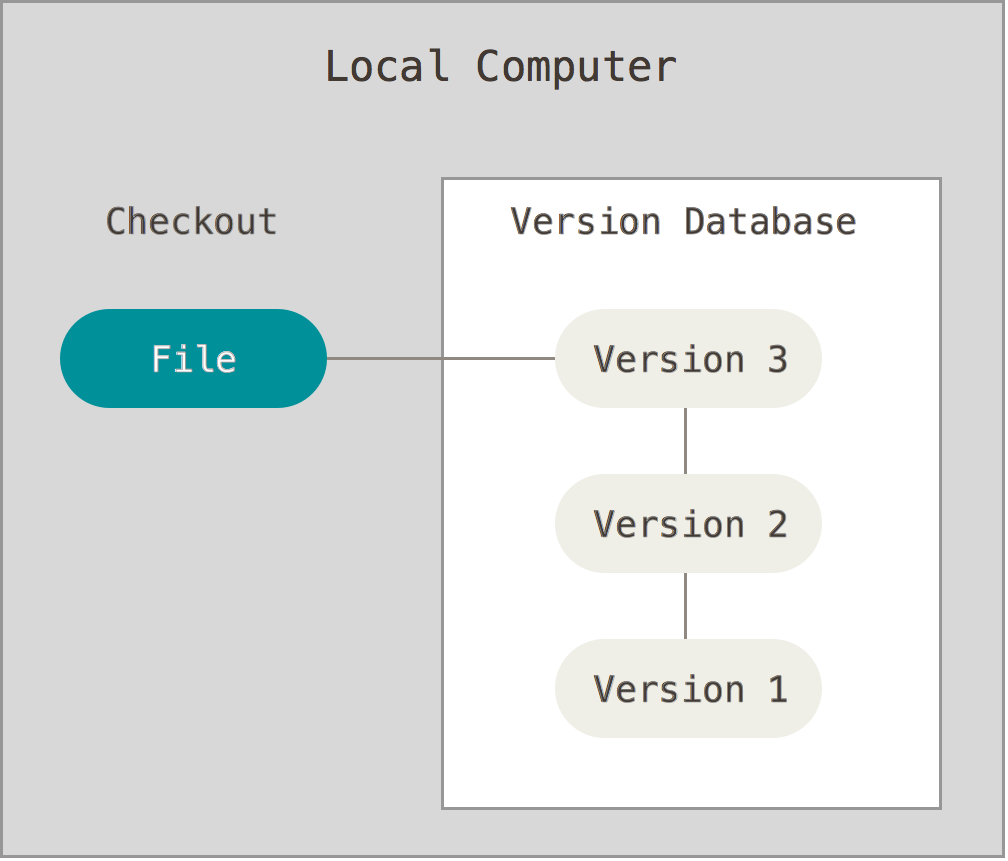
\includegraphics{images/local}
  \caption{Gestion de version locale}
  \label{fig:progit:local}
\end{figure}

Un des systèmes les plus populaires était RCS, qui est encore distribué avec de nombreux systèmes d'exploitation aujourd'hui.
Même le système d'exploitation populaire Mac OS X inclut le programme `rcs` lorsqu'on installe les outils de développement logiciel.
Cet outil fonctionne en conservant des ensembles de patchs (c'est-à-dire la différence entre les fichiers) d'une version à l'autre dans un format spécial sur disque ;
il peut alors restituer l'état de n'importe quel fichier à n'importe quel instant en ajoutant toutes les différences.

\subsubsection{Les systèmes de gestion de version centralisés}


Le problème majeur que les gens rencontrent est qu'ils ont besoin de collaborer avec des développeurs sur d'autres ordinateurs.
Pour traiter ce problème, les systèmes de gestion de version centralisés (CVCS en anglais pour \emph{Centralized Version Control Systems}) furent développés.
Ces systèmes tels que CVS, Subversion, et Perforce, mettent en place un serveur central qui contient tous les fichiers sous gestion de version, et des clients qui peuvent extraire les fichiers de ce dépôt central.
Pendant de nombreuses années, cela a été le standard pour la gestion de version.

\begin{figure}[h]
  \centering
  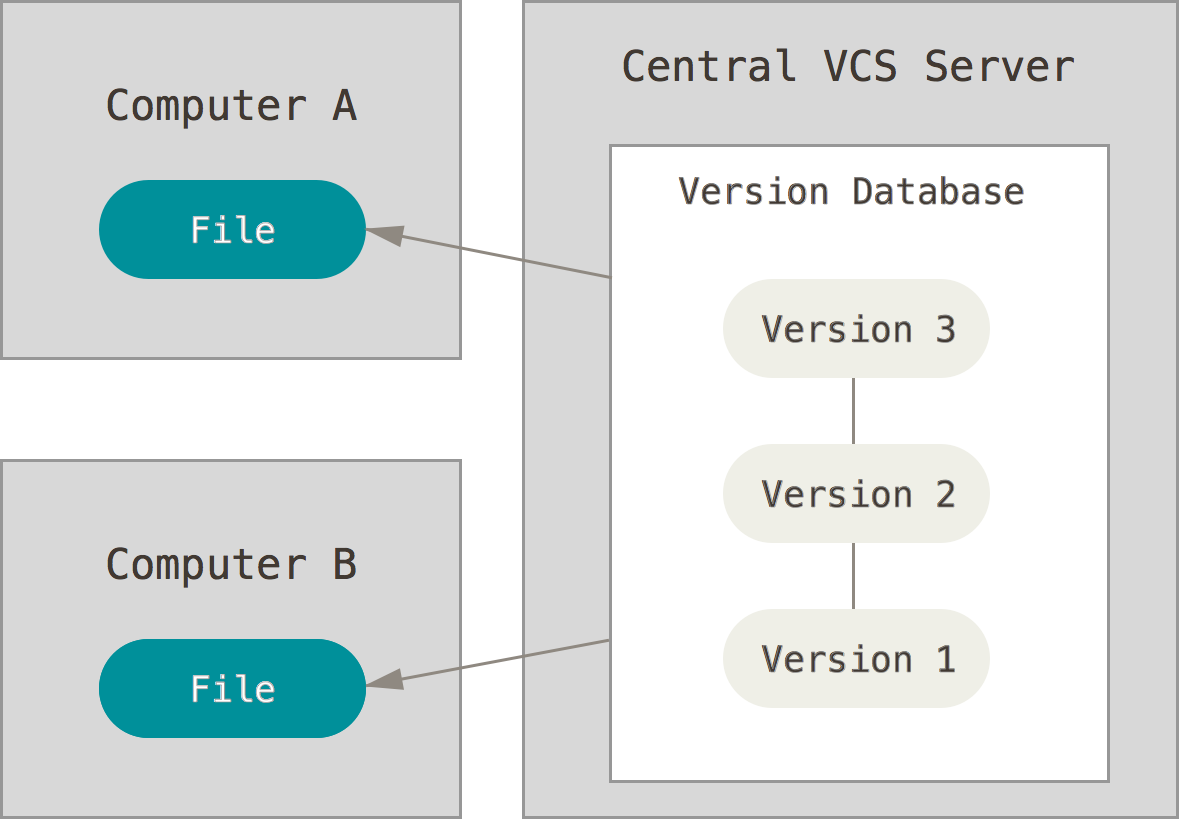
\includegraphics{images/centralized}
  \caption{Gestion de version centralisée}
  \label{fig:progit:centralized}
\end{figure}

Ce schéma offre de nombreux avantages par rapport à la gestion de version locale.
Par exemple, chacun sait jusqu'à un certain point ce que tous les autres sont en train de faire sur le projet.
Les administrateurs ont un contrôle fin des permissions et il est beaucoup plus facile d'administrer un CVCS que de gérer des bases de données locales.

Cependant ce système a aussi de nombreux défauts.
Le plus visible est le point unique de panne que le serveur centralisé représente.
Si ce serveur est en panne pendant une heure, alors durant cette heure, aucun client ne peut collaborer ou enregistrer les modifications issues de son travail.
Si le disque dur du serveur central se corrompt, et s'il n'y a pas eu de sauvegarde, vous perdez absolument tout de l'historique d'un projet en dehors des sauvegardes locales que les gens auraient pu réaliser sur leurs machines locales.
Les systèmes de gestion de version locaux souffrent du même problème — dès qu'on a tout l'historique d'un projet sauvegardé à un endroit unique, on prend le risque de tout perdre.

\subsubsection{Les systèmes de gestion de version distribués}

C'est à ce moment que les systèmes de gestion de version distribués entrent en jeu (DVCS en anglais pour \emph{Distributed Version Control Systems}).
Dans un DVCS (tel que Git, Mercurial, Bazaar ou Darcs), les clients n'extraient plus seulement la dernière version d'un fichier, mais ils dupliquent complètement le dépôt.
Ainsi, si le serveur disparaît et si les systèmes collaboraient via ce serveur, n'importe quel dépôt d'un des clients peut être copié sur le serveur pour le restaurer.
Chaque extraction devient une sauvegarde complète de toutes les données.

\begin{figure}[h]
  \centering
  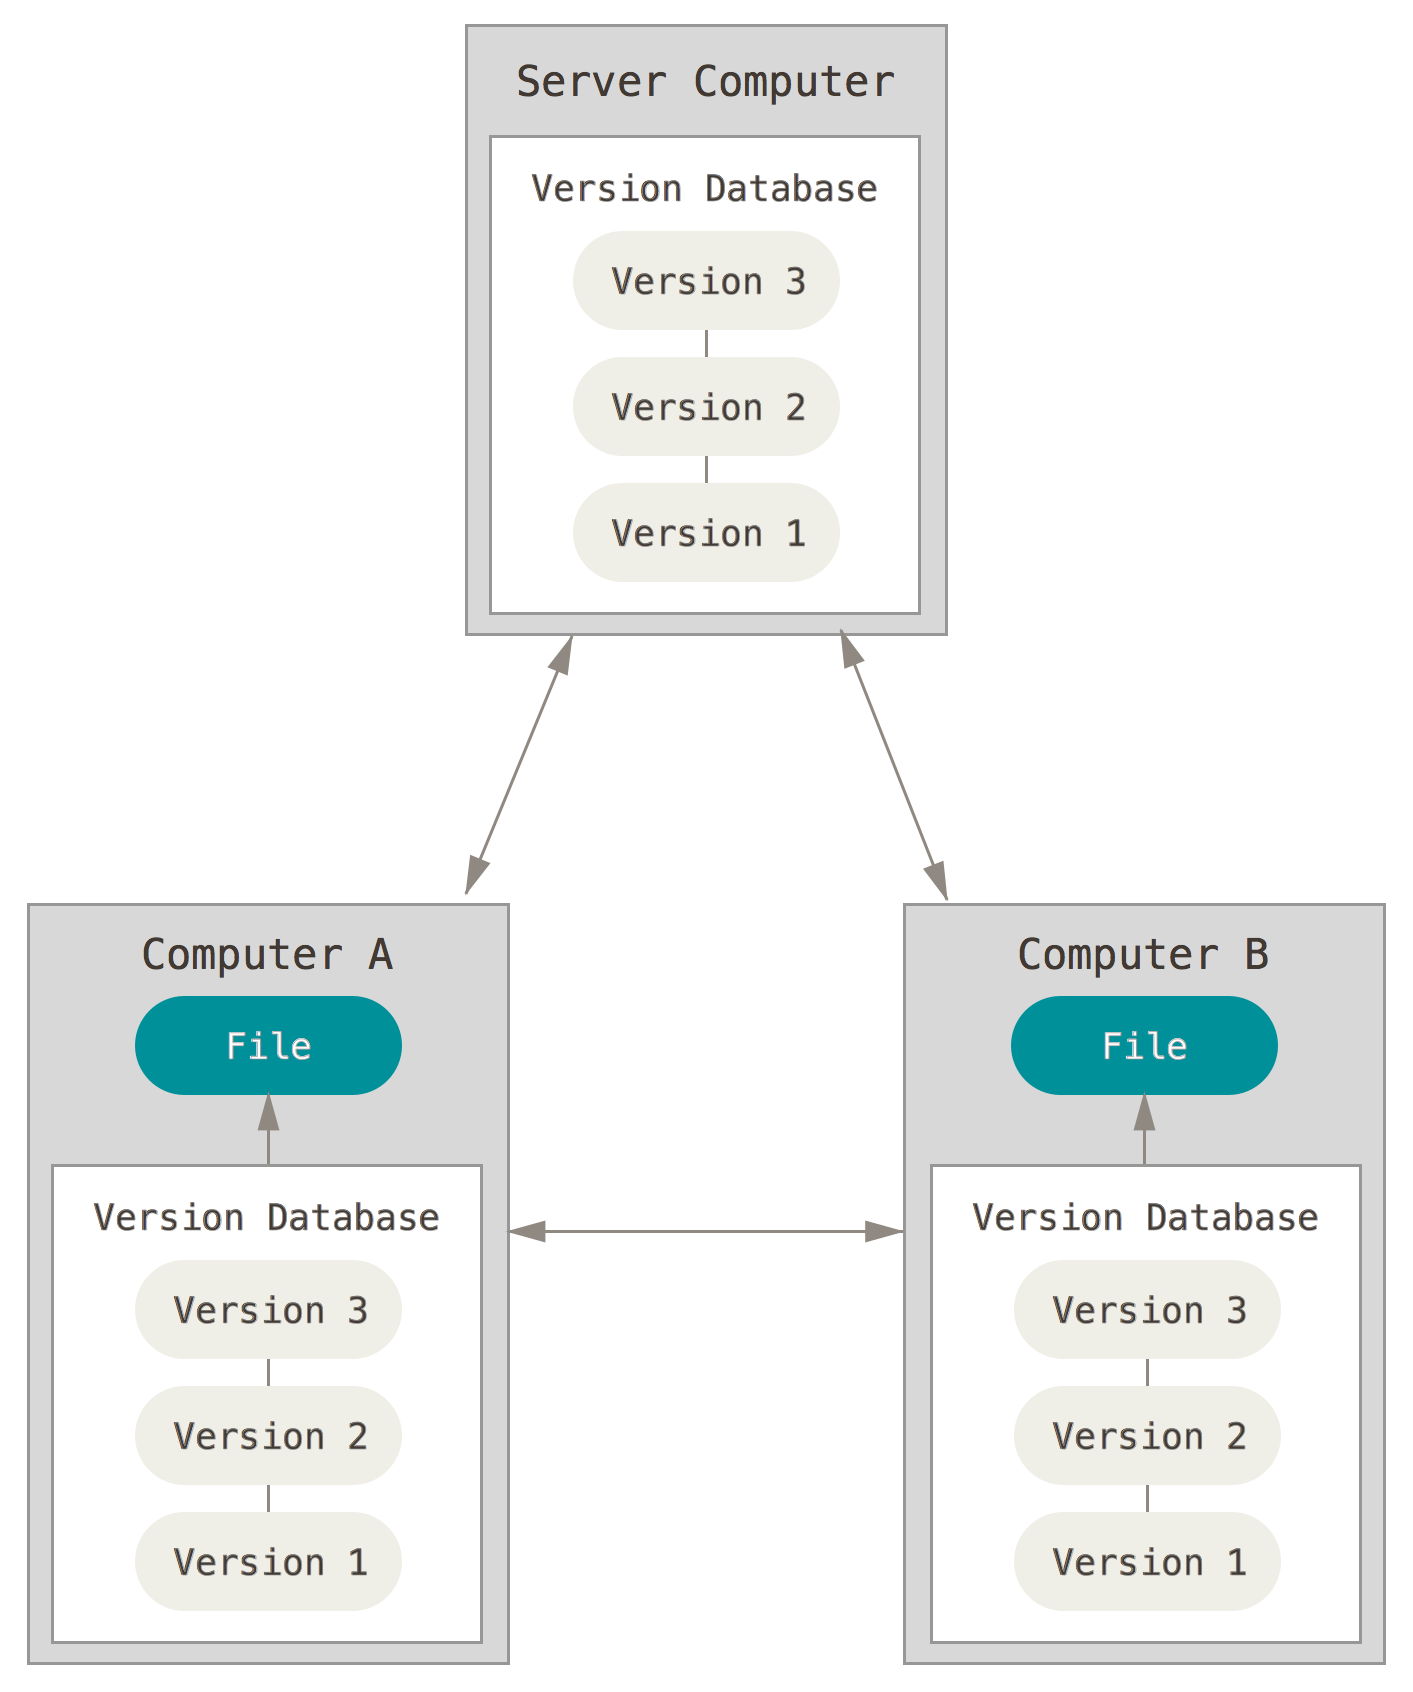
\includegraphics{images/distributed}
  \caption{Gestion de version distribuée}
  \label{fig:progit:distributed}
\end{figure}

De plus, un grand nombre de ces systèmes gère particulièrement bien le fait d'avoir plusieurs dépôts avec lesquels travailler, vous permettant de collaborer avec différents groupes de personnes de manières différentes simultanément dans le même projet.
Cela permet la mise en place de différentes chaînes de traitement qui ne sont pas réalisables avec les systèmes centralisés, tels que les modèles hiérarchiques.

\subsection{Une rapide histoire de Git}

Comme de nombreuses choses extraordinaires de la vie, Git est né avec une dose de destruction créative et de controverse houleuse.
Le noyau Linux est un projet libre de grande envergure.
Pour la plus grande partie de sa vie (1991–2002), les modifications étaient transmises sous forme de patchs et d'archives de fichiers.
En 2002, le projet du noyau Linux commença à utiliser un DVCS propriétaire appelé BitKeeper.

En 2005, les relations entre la communauté développant le noyau Linux et la société en charge du développement de BitKeeper furent rompues, et le statut de gratuité de l'outil fut révoqué.
Cela poussa la communauté du développement de Linux (et plus particulièrement Linus Torvalds, le créateur de Linux) à développer son propre outil en se basant sur les leçons apprises lors de l'utilisation de BitKeeper.
Certains des objectifs du nouveau système étaient les suivants :

\begin{itemize}
\item vitesse ;
\item conception simple ;
\item support pour les développements non linéaires (milliers de branches parallèles) ;
\item complètement distribué ;
\item capacité à gérer efficacement des projets d'envergure tels que le noyau Linux (vitesse et compacité des données)
\end{itemize}

Depuis sa naissance en 2005, Git a évolué et mûri pour être facile à utiliser tout en conservant ses qualités initiales.
Il est incroyablement rapide, il est très efficace pour de grands projets et il a un incroyable système de branches pour des développements non linéaires (voir la \autoref{sec:git:branching}).

\subsection{Rudiments de Git}

Donc, qu'est-ce que Git en quelques mots ?
Il est important de bien comprendre cette section, parce que si on comprend la nature de Git et les principes sur lesquels il repose, alors utiliser efficacement Git devient simple.
Au cours de l'apprentissage de Git, essayez de libérer votre esprit de ce que vous pourriez connaître d'autres VCS, tels que Subversion et Perforce ;
ce faisant, vous vous éviterez de petites confusions à l'utilisation de cet outil.
Git enregistre et gère l'information très différemment des autres systèmes, même si l'interface utilisateur paraît similaire ;
comprendre ces différences vous évitera des surprises.

\subsubsection{Des instantanés, pas des différences}

La différence majeure entre Git et les autres VCS (Subversion et autres) réside dans la manière dont Git considère les données.
Au niveau conceptuel, la plupart des autres systèmes gèrent l'information comme une liste de modifications de fichiers.
Ces systèmes (CVS, Subversion, Perforce, Bazaar et autres) considèrent l'information qu'ils gèrent comme une liste de fichiers et les modifications effectuées sur chaque fichier dans le temps.

\begin{figure}[h]
  \centering
  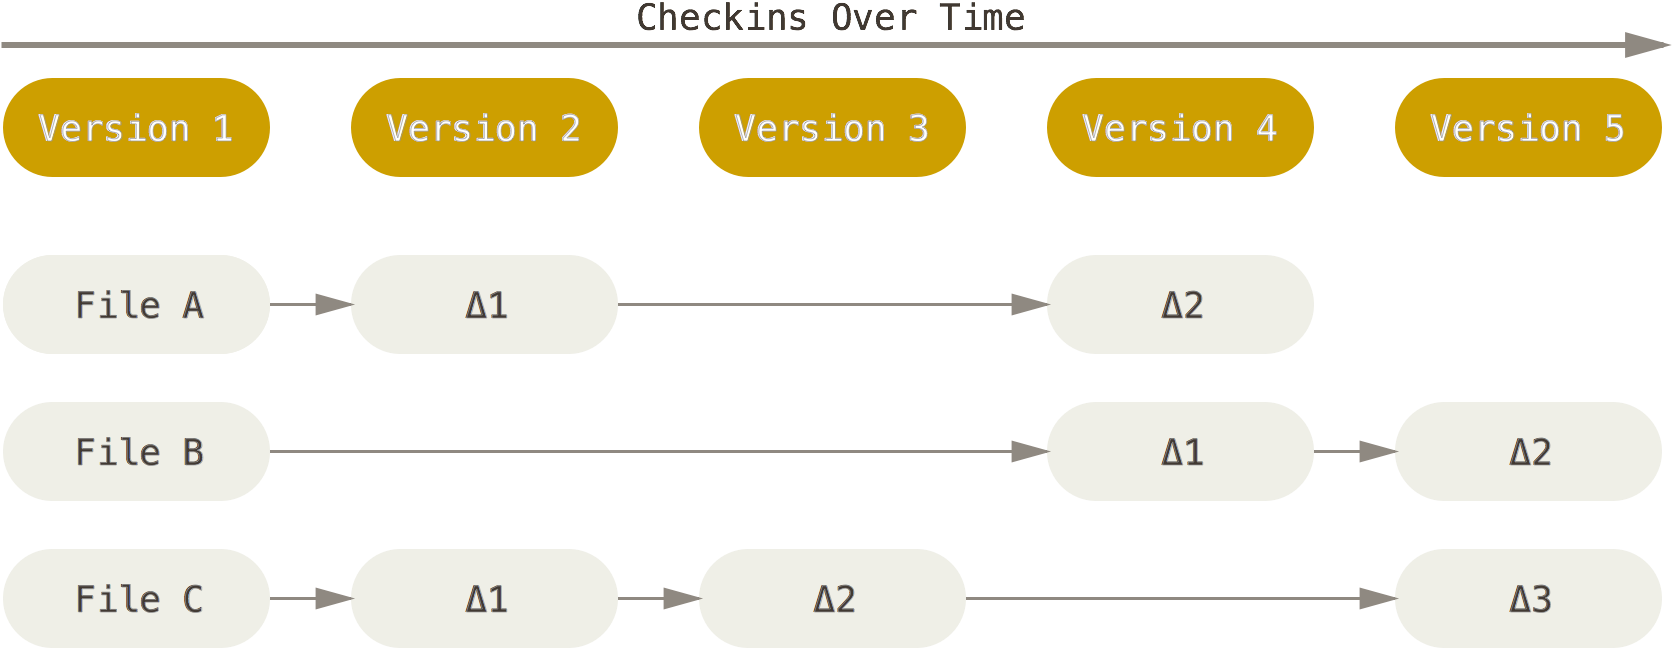
\includegraphics{images/deltas}
  \caption{D'autres systèmes sauvent l'information comme des modifications sur des fichiers}
  \label{fig:progit:deltas}
\end{figure}

Git ne gère pas et ne stocke pas les informations de cette manière.
À la place, Git pense ses données plus comme un instantané d'un mini système de fichiers.
À chaque fois que vous validez ou enregistrez l'état du projet dans Git, il prend effectivement un instantané du contenu de votre espace de travail à ce moment et enregistre une référence à cet instantané.
Pour être efficace, si les fichiers n'ont pas changé, Git ne stocke pas le fichier à nouveau, juste une référence vers le fichier original qu'il a déjà enregistré.
Git pense ses données plus à la manière d'un *flux d'instantanés*.

\begin{figure}[h]
  \centering
  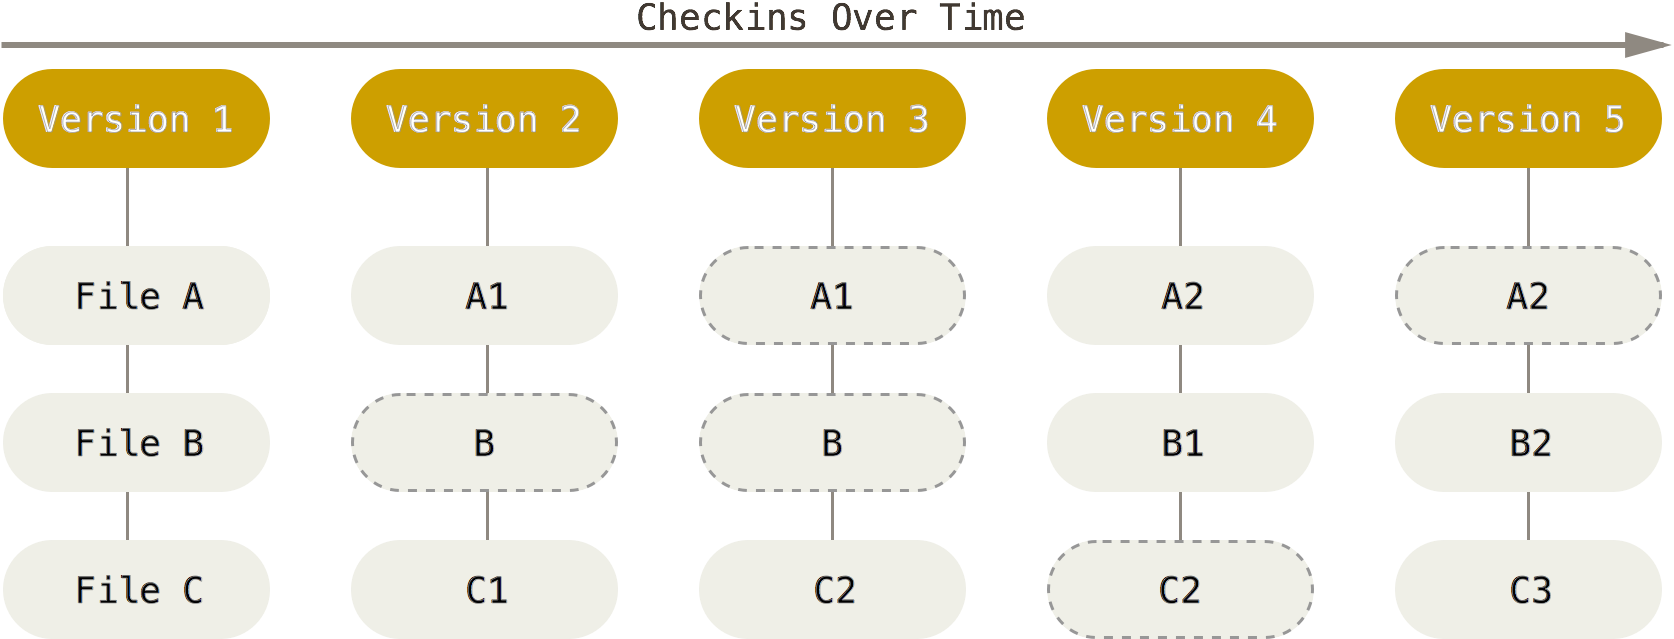
\includegraphics{images/snapshots}
  \caption{Git stocke les données comme des instantanés du projet au cours du temps}
  \label{fig:progit:snapshots}
\end{figure}

C'est une distinction importante entre Git et quasiment tous les autres VCS.
Git a reconsidéré quasiment tous les aspects de la gestion de version que la plupart des autres systèmes ont copiés des générations précédentes.
Git ressemble beaucoup plus à un mini système de fichiers avec des outils incroyablement puissants construits dessus, plutôt qu'à un simple VCS.
Nous explorerons les bénéfices qu'il y a à penser les données de cette manière quand nous aborderons la gestion de branches dans la \autoref{sec:git:branching}.

\subsubsection{Presque toutes les opérations sont locales}

La plupart des opérations de Git ne nécessitent que des fichiers et ressources locaux — généralement aucune information venant d'un autre ordinateur du réseau n'est nécessaire.
Si vous êtes habitué à un CVCS où toutes les opérations sont ralenties par la latence des échanges réseau, cet aspect de Git vous fera penser que les dieux de la vitesse ont octroyé leurs pouvoirs à Git.
Comme vous disposez de l'historique complet du projet localement sur votre disque dur, la plupart des opérations semblent instantanées.

Par exemple, pour parcourir l'historique d'un projet, Git n'a pas besoin d'aller le chercher sur un serveur pour vous l'afficher ;
il n'a qu'à simplement le lire directement dans votre base de données locale.
Cela signifie que vous avez quasi-instantanément accès à l'historique du projet.
Si vous souhaitez connaître les modifications introduites entre la version actuelle d'un fichier et son état un mois auparavant, Git peut rechercher l'état du fichier un mois auparavant et réaliser le calcul de différence, au lieu d'avoir à demander cette différence à un serveur ou de devoir récupérer l'ancienne version sur le serveur pour calculer la différence localement.

Cela signifie aussi qu'il y a très peu de choses que vous ne puissiez réaliser si vous n'êtes pas connecté ou hors VPN.
Si vous voyagez en train ou en avion et voulez avancer votre travail, vous pouvez continuer à gérer vos versions sans soucis en attendant de pouvoir de nouveau vous connecter pour partager votre travail.
Si vous êtes chez vous et ne pouvez avoir une liaison VPN avec votre entreprise, vous pouvez tout de même travailler.
Pour de nombreux autres systèmes, faire de même est impossible ou au mieux très contraignant.
Avec Perforce par exemple, vous ne pouvez pas faire grand-chose tant que vous n'êtes pas connecté au serveur.
Avec Subversion ou CVS, vous pouvez éditer les fichiers, mais vous ne pourrez pas soumettre des modifications à votre base de données (car celle-ci est sur le serveur non accessible).
Cela peut sembler peu important a priori, mais vous seriez étonné de découvrir quelle grande différence cela peut constituer à l'usage.

\subsubsection{Git gère l'intégrité}

Dans Git, tout est vérifié par une somme de contrôle avant d'être stocké et par la suite cette somme de contrôle, signature unique, sert de référence.
Cela signifie qu'il est impossible de modifier le contenu d'un fichier ou d'un répertoire sans que Git ne s'en aperçoive.
Cette fonctionnalité est ancrée dans les fondations de Git et fait partie intégrante de sa philosophie.
Vous ne pouvez pas perdre des données en cours de transfert ou corrompre un fichier sans que Git ne puisse le détecter.

Le mécanisme que Git utilise pour réaliser les sommes de contrôle est appelé une empreinte SHA-1.
C'est une chaîne de caractères composée de 40 caractères hexadécimaux (de $0$ à $9$ et de «a» à «f») calculée en fonction du contenu du fichier ou de la structure du répertoire considéré.
Une empreinte SHA-1 ressemble à ceci :
\begin{Schunk}
\begin{Verbatim}
24b9da6552252987aa493b52f8696cd6d3b00373
\end{Verbatim}
\end{Schunk}

Vous trouverez ces valeurs à peu près partout dans Git car il les utilise pour tout.
En fait, Git stocke tout non pas avec des noms de fichiers, mais dans la base de données Git indexée par ces valeurs.

\subsubsection{Généralement, Git ne fait qu'ajouter des données}

Quand vous réalisez des actions dans Git, la quasi-totalité d'entre elles ne font qu'ajouter des données dans la base de données de Git.
Il est très difficile de faire réaliser au système des actions qui ne soient pas réversibles ou de lui faire effacer des données d'une quelconque manière.
Par contre, comme dans la plupart des systèmes de gestion de version, vous pouvez perdre ou corrompre des modifications qui n'ont pas encore été entrées en base ;
mais dès que vous avez validé un instantané dans Git, il est très difficile de le perdre, spécialement si en plus vous synchronisez votre base de données locale avec un dépôt distant.

Cela fait de l'usage de Git un vrai plaisir, car on peut expérimenter sans danger de casser définitivement son projet.
Pour une information plus approfondie sur la manière dont Git stocke ses données et comment récupérer des données qui pourraient sembler perdues, référez-vous à la \autoref{sec:git:undoing}.

\subsubsection{Les trois états}

Un peu de concentration maintenant.
Il est primordial de se souvenir de ce qui suit si vous souhaitez que le reste de votre apprentissage s'effectue sans difficulté.
Git gère trois états dans lesquels les fichiers peuvent résider : validé, modifié et indexé.
Validé signifie que les données sont stockées en sécurité dans votre base de données locale.
Modifié signifie que vous avez modifié le fichier mais qu'il n'a pas encore été validé en base.
Indexé signifie que vous avez marqué un fichier modifié dans sa version actuelle pour qu'il fasse partie du prochain instantané du projet.

Ceci nous mène aux trois sections principales d'un projet Git : le répertoire Git, le répertoire de travail et la zone d'index.

\begin{figure}[h]
  \centering
  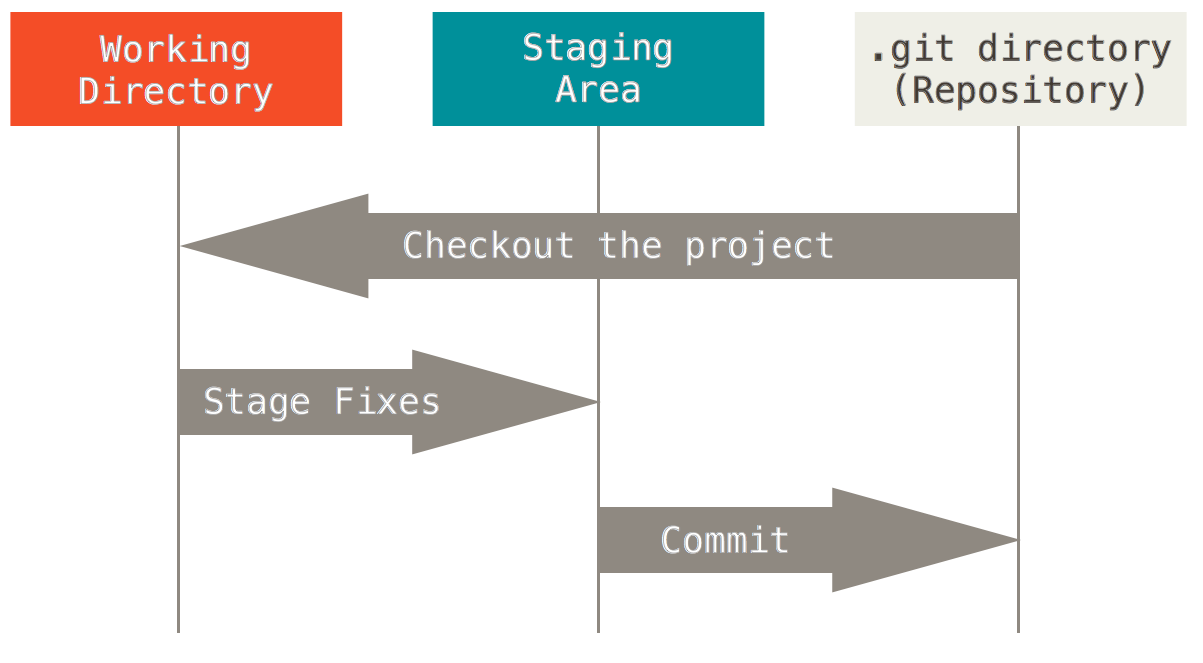
\includegraphics{images/areas}
  \caption{Répertoire de travail, zone d'index et répertoire Git}
  \label{fig:progit:areas}
\end{figure}

Le répertoire Git est l'endroit où Git stocke les méta-données et la base de données des objets de votre projet.
C'est la partie la plus importante de Git, et c'est ce qui est copié lorsque vous clonez un dépôt depuis un autre ordinateur.

Le répertoire de travail est une extraction unique d'une version du projet.
Ces fichiers sont extraits depuis la base de données compressée dans le répertoire Git et placés sur le disque pour pouvoir être utilisés ou modifiés.

La zone d'index est un simple fichier, généralement situé dans le répertoire Git, qui stocke les informations concernant ce qui fera partie du prochain instantané. On l'appelle aussi des fois la zone de préparation.

L'utilisation standard de Git se passe comme suit :
\begin{enumerate}
\item vous modifiez des fichiers dans votre répertoire de travail ;
\item vous indexez les fichiers modifiés, ce qui ajoute des instantanés de ces fichiers dans la zone d'index ;
\item vous validez, ce qui a pour effet de basculer les instantanés des fichiers de l'index dans la base de données du répertoire Git.
\end{enumerate}

Si une version particulière d'un fichier est dans le répertoire Git, il est considéré comme validé.
S'il est modifié mais a été ajouté dans la zone d'index, il est indexé.
S'il a été modifié depuis le dernier instantané mais n'a pas été indexé, il est modifié.
Dans la \autoref{sec:git:git_basics}, vous en apprendrez plus sur ces états et comment vous pouvez en tirer parti ou complètement occulter la phase d'indexation.

\subsection{La ligne de commande}

Il existe de nombreuses manières différentes d'utiliser Git.
Il y a les outils originaux en ligne de commande et il y a de nombreuses interfaces graphiques avec des capacités variables.
Dans ce livre, nous utiliserons Git en ligne de commande.
Tout d'abord, la ligne de commande est la seule interface qui permet de lancer \emph{toutes} les commandes Git --- la plupart des interfaces graphiques simplifient l'utilisation en ne couvrant qu'un sous-ensemble des fonctionnalités de Git.
Si vous savez comment utiliser la version en ligne de commande, vous serez à même de comprendre comment fonctionne la version graphique, tandis que l'inverse n'est pas nécessairement vrai.
De plus, le choix d'un outil graphique est sujet à des goûts personnels, mais \emph{tous} les utilisateurs auront les commandes en lignes installées et utilisables.

Nous considérons que vous savez ouvrir un Terminal sous Mac ou une invite de commandes ou Powershell sous Windows.
Si ce n'est pas le cas, il va falloir tout d'abord vous renseigner sur ces applications pour pouvoir comprendre la suite des exemples et descriptions du livre.

\subsection{Installation de Git}

Avant de commencer à utiliser Git, il faut qu'il soit disponible sur votre ordinateur.
Même s'il est déjà installé, c'est probablement une bonne idée d'utiliser la dernière version disponible.
Vous pouvez l'installer soit comme paquet ou avec un installateur, soit en téléchargeant le code et en le compilant par vous-même.

\warningbox{Ce livre a été écrit en utilisant Git version *2.0.0*.
  Bien que la plupart des commandes utilisées fonctionnent vraisemblablement encore avec d'anciennes version de Git, certaines peuvent agir différemment.
  Comme Git est particulièrement excellent pour préserver les compatibilités amont, toute version supérieure à 2.0 devrait fonctionner sans différence.}

\subsubsection{Installation sur Linux}

Si vous voulez installer les outils basiques de Git sur Linux via un installateur binaire, vous pouvez généralement le faire au moyen de l'outil de gestion de paquet fourni avec votre distribution.
Sur Fedora, par exemple, vous pouvez utiliser \code{dnf}:
\begin{Schunk}
\begin{Verbatim}
$ dnf install git-all
\end{Verbatim}
\end{Schunk}

Sur une distribution basée sur Debian, telle que Ubuntu, essayer \code{apt-get}:
\begin{Schunk}
\begin{Verbatim}
$ apt-get install git-all
\end{Verbatim}
\end{Schunk}

Pour plus d'options, des instructions d'installation sur différentes versions Unix sont disponibles sur le site web de Git, à \link{http://git-scm.com/download/linux}{}.

\subsubsection{Installation sur Mac}

Il existe plusieurs méthodes d'installation de Git sur un Mac.
La plus facile est probablement d'installer les \emph{Xcode Command Line Tools}.
Sur Mavericks (10.9) ou postérieur, vous pouvez simplement essayer de lancer \code{git} dans le terminal la première fois.
S'il n'est pas déjà installé, il vous demandera de le faire.

Si vous souhaitez une version plus à jour, vous pouvez aussi l'installer à partir de l'installateur binaire.
Un installateur de Git pour OS X est maintenu et disponible au téléchargement sur le site web de Git à \link{http://git-scm.com/download/mac}{}.

Vous pouvez aussi l'installer comme sous-partie de l'installation de GitHub pour Mac.
Leur outil Git graphique a une option pour installer les outils en ligne de commande.
Vous pouvez télécharger cet outil depuis le site web de GitHub pour Mac, à \link{http://mac.github.com}{}.

\subsubsection{Installation sur Windows}

Il existe aussi plusieurs manières d'installer Git sur Windows.
L'application officielle est disponible au téléchargement sur le site web de Git.
Rendez-vous sur http://git-scm.com/download/win[] et le téléchargement démarrera automatiquement.
Notez que c'est un projet nommé \emph{Git for Windows} (appelé aussi msysGit), qui est séparé de Git lui-même; pour plus d'information, rendez-vous à \link{http://msysgit.github.io/}{}.

Une autre méthode facile pour installer Git est d'installer \emph{Github for Windows}.
L'installateur inclut une version en ligne de commande avec l'interface graphique.
Elle fonctionne aussi avec Powershell et paramètre correctement les caches d'authentification et les réglages CRLF.
Nous en apprendrons plus sur ces sujets plus tard, mais il suffit de savoir que ces options sont très utiles.
Vous pouvez télécharger ceci depuis le site de \emph{Github for Windows}, à l'adresse \link{http://windows.github.com}{}.

\subsubsection{Installation depuis les sources}

Certains peuvent plutôt trouver utile d'installer Git depuis les sources car on obtient la version la plus récente.
Les installateurs de version binaire tendent à être un peu en retard, même si Git a gagné en maturité ces dernières années, ce qui limite les évolutions.

Pour installer Git, vous avez besoin des bibliothèques suivantes: autotools, curl, zlib, openssl, expat, libiconv.
Par exemple, si vous avez un système d'exploitation qui utilise dnf (tel que Fedora) ou apt-get (tel qu'un système basé sur Debian), vous pouvez utiliser l'une des commandes suivantes pour installer les dépendances:

\begin{Schunk}
\begin{Verbatim}
$ dnf install curl-devel expat-devel gettext-devel \
    openssl-devel zlib-devel
\end{Verbatim}
\end{Schunk}

\begin{Schunk}
\begin{Verbatim}
$ apt-get install libcurl4-gnutls-dev libexpat1-dev gettext \
    libz-dev libssl-dev
\end{Verbatim}
\end{Schunk}

Quand vous avez toutes les dépendances nécessaires, vous pouvez poursuivre et télécharger la dernière version de Git depuis plusieurs sites.
Vous pouvez l'obtenir via Kernel.org, à \link{https://www.kernel.org/pub/software/scm/git}{}, ou sur le miroir sur le site web GitHub à \link{https://github.com/git/git/releases}{}.

Puis, compiler et installer:

\begin{Schunk}
\begin{Verbatim}
$ tar -zxf git-1.9.1.tar.gz
$ cd git-1.9.1
$ make configure
$ ./configure --prefix=/usr
$ make all doc info
$ sudo make install install-doc install-html install-info
\end{Verbatim}
\end{Schunk}

Après ceci, vous pouvez obtenir Git par Git lui-même pour les mises à jour:

\begin{Schunk}
\begin{Verbatim}
$ git clone git://git.kernel.org/pub/scm/git/git.git
\end{Verbatim}
\end{Schunk}

\subsection{Paramétrage à la première utilisation de Git}
\label{sec:git:first_time}

Maintenant que vous avez installé Git sur votre système, vous voudrez personnaliser votre environnement Git.
Vous ne devriez avoir à réaliser ces réglages qu'une seule fois;
ils persisteront lors des mises à jour.
Vous pouvez aussi les changer à tout instant en relançant les mêmes commandes.

Git contient un outil appelé \code{git config} pour vous permettre de voir et modifier les variables de configuration qui contrôlent tous les aspects de l'apparence et du comportement de Git.
Ces variables peuvent être stockées dans trois endroits différents:
\begin{itemize}
\item Fichier \code{/etc/gitconfig}: Contient les valeurs pour tous les utilisateurs et tous les dépôts du système.
Si vous passez l'option \code{--system} à \code{git config}, il lit et écrit ce fichier spécifiquement.
\item Fichier \verb=~/.gitconfig=: Spécifique à votre utilisateur.
Vous pouvez forcer Git à lire et écrire ce fichier en passant l'option \code{--global}.
\item Fichier \code{config} dans le répertoire Git (c'est-à-dire \code{.git/config}) du dépôt en cours d'utilisation: spécifique au seul dépôt en cours.
\end{itemize}
Chaque niveau surcharge le niveau précédent, donc les valeurs dans \code{.git/config} surchargent celles de \code{/etc/gitconfig}.

Sur les systèmes Windows, Git recherche le fichier \code{.gitconfig} dans le répertoire \code{\$HOME} (\code{\%USERPROFILE\%} dans l’environnement natif de Windows) qui est \code{C:{\bs}Documents and Settings{\bs}\$USER} ou \code{C:{\bs}Users{\bs}\$USER} la plupart du temps, selon la version (\code{\$USER} devient \code{\%USERNAME\%} dans l’environnement de Windows).
Il recherche tout de même \code{/etc/gitconfig}, bien qu'il soit relatif à la racine MSys, qui se trouve où vous aurez décidé d'installer Git sur votre système Windows.
Si vous utilisez une version 2.x ou supérieure de Git pour Windows, il y a aussi un fichier de configuration système à \code{C:{\bs}Documents and Settings{\bs}All Users{\bs}Application Data{\bs}Git{\bs}config} sur Windows XP, et dans \code{C:{\bs}ProgramData{\bs}Git{\bs}config} sur Windows Vista et supérieur.
Ce fichier de configuration ne peut être modifié qu'avec la commande \code{git config -f \meta{fichier}} en tant qu'administrateur.

\subsubsection{Votre identité}

La première chose à faire après l'installation de Git est de renseigner votre nom et votre adresse de courriel.
C'est une information importante car toutes les validations dans Git utilisent cette information et elle est indélébile dans toutes les validations que vous pourrez réaliser:
\begin{Schunk}
\begin{Verbatim}
$ git config --global user.name "John Doe"
$ git config --global user.email johndoe@example.com
\end{Verbatim}
\end{Schunk}

Encore une fois, cette étape n'est nécessaire qu'une fois si vous passez l'option \code{--global}, parce que Git utilisera toujours cette information pour tout ce que votre utilisateur fera sur ce système.
Si vous souhaitez surcharger ces valeurs avec un nom ou une adresse de courriel différents pour un projet spécifique, vous pouvez lancer ces commandes sans option \code{--global} lorsque vous êtes dans ce projet.

De nombreux outils graphiques vous aideront à le faire la première fois que vous les lancerez.

\subsubsection{Votre éditeur de texte}

À présent que votre identité est renseignée, vous pouvez configurer l'éditeur de texte qui sera utilisé quand Git vous demande de saisir un message.
Par défaut, Git utilise l'éditeur configuré au niveau système, qui est généralement Vi ou Vim.
Si vous souhaitez utiliser un éditeur de texte différent, comme Emacs, vous pouvez entrer ce qui suit:
\begin{Schunk}
\begin{Verbatim}
$ git config --global core.editor emacs
\end{Verbatim}
\end{Schunk}

\cautionbox{Vim et Emacs sont des éditeurs de texte populaires chez les développeurs sur les systèmes à base Unix tels que Linux et Mac.
Si vous n'êtes habitué à aucun de ces deux éditeurs ou utilisez un système Windows, il se peut que vous deviez chercher les instructions pour renseigner votre éditeur favori.
Si vous ne renseignez pas un éditeur et ne connaissez pas Vim ou Emacs, vous risquez fort d'avoir des surprises lorsqu'ils démarreront.}

\subsubsection{Vérifier vos paramètres}

Si vous souhaitez vérifier vos réglages, vous pouvez utiliser la commande \code{git config --list} pour lister tous les réglages que Git a pu trouver jusqu'ici:
\begin{Schunk}
\begin{Verbatim}
$ git config --list
user.name=John Doe
user.email=johndoe@example.com
color.status=auto
color.branch=auto
color.interactive=auto
color.diff=auto
...
\end{Verbatim}
\end{Schunk}

Vous pourrez voir certains paramètres apparaître plusieurs fois car Git lit les mêmes paramètres depuis plusieurs fichiers (\code{/etc/gitconfig} et \verb=~/.gitconfig=, par exemple).
Git utilise la dernière valeur pour chaque paramètre.

Vous pouvez aussi vérifier la valeur effective d'un paramètre particulier en tapant \code{git config \meta{paramètre}}:
\begin{Schunk}
\begin{Verbatim}
$ git config user.name
John Doe
\end{Verbatim}
\end{Schunk}

\subsection{Obtenir de l'aide}
\label{sec:git:help}

Si vous avez besoin d'aide pour utiliser Git, il y a trois moyens d'obtenir les pages de manuel pour toutes les commandes de Git:

\begin{Schunk}
\begin{Verbatim}
$ git help <commande>
$ git <commande> --help
$ man git-<commande>
\end{Verbatim}
\end{Schunk}

Par exemple, vous pouvez obtenir la page de manuel pour la commande \code{config} en lançant:
\begin{Schunk}
\begin{Verbatim}
$ git help config
\end{Verbatim}
\end{Schunk}

Ces commandes sont vraiment sympathiques car vous pouvez y accéder depuis partout, y compris hors connexion.
Si les pages de manuel et ce livre ne sont pas suffisants, vous pouvez essayer les canaux \code{\#git} ou \code{\#github} sur le serveur IRC Freenode (\code{irc.freenode.net}).
Ces canaux sont régulièrement peuplés de centaines de personnes qui ont une bonne connaissance de Git et sont souvent prêtes à aider.

\subsection{Résumé}

Vous devriez avoir à présent une compréhension initiale de ce que Git est et en quoi il est différent des CVCS que vous pourriez déjà avoir utilisés.
Vous devriez aussi avoir une version de Git en état de fonctionnement sur votre système, paramétrée avec votre identité.
Il est temps d'apprendre les bases d'utilisation de Git.


%%% Local Variables:
%%% mode: latex
%%% TeX-engine: xetex
%%% TeX-master: "programmer-avec-r"
%%% coding: utf-8
%%% End:
